\apendice{Procesado automático de la imagen}
\label{anexo:F}
\section{Introducción}
En este apartado vamos a explicar lo que hemos investigado sobre la detección de bordes para el modo automático.

Esto lo vamos afrontar desde dos puntos de vista, el primero será por el procesado de imágenes, esto consistirá en binarizar la imagen usando un kernel conocido y observar si los resultados nos muestran algún resultado factible.
Como segunda opción vamos a intentar ejecutar algoritmos de Deep Learning para ver si mejora el resultado usando estos algoritmos.

Para entender este anexo y este procesado, por lo menos es necesario haberse leído los conceptos teóricos y herramientas mencionadas en la memoria ya que no se ha duplicado dicha información en varios sitios.

\section{Extracción de bordes mediante procesado de imagen}
Esta sección consistirá, partiendo de una imagen en extraer las características, en este caso será la detección de los bordes contenidos, se corresponderán con las estrías que queremos detectar. Lo vamos a detectar a partir de los métodos explicados a continuación. 

A todas las imágenes se las va a aplicar un proceso de convolución, con el Kernel \cite{wiki:kernels} específico en cada caso.

Una convolución es una operación matemática, que no es la multiplicación de matrices tradicional, es el proceso de agregar cada porción de la imagen a sus vecinos locales ponderado por el Kernel. 
Este proceso no solo vale para detectar bordes, tiene estas otras aplicaciones.
\begin{itemize}
\item Detección de bordes: Detectar los puntos donde acaba un objeto y empieza otro, también las aristas o bordes de las imágenes.
\item Desenfoques y difuminado: Desenfocar o difuminar la imagen a partir de hacer la operación de convolución con una máscara diseñada para ello.
\item Eliminar ruido: Sirve para moderar los valores de la imagen  y hacer que estén mas centrados en un rango y así eliminar el ruido aleatorio. 
\end{itemize}

\subsection{Laplace:}
Esta función busca bordes usando el operador de Laplace \cite{wiki:Laplace}. En nuestro caso de tamaño 3 (ya que se puede especificar el tamaño).
Se ilustra el Kernel de Laplace en la figura~\ref{F_k1}.


Observaciones:
Como se ilustra en la figura~\ref{fig:1.1.1}, no es un método válido para nuestro propósito, porque no detecta los bordes, simplemente deja algunas partes difuminadas, pero nada sobre lo que podamos trabajar para obtener la imagen binarizada. Por lo que no vamos a continuar usándolo.

\subsection{Prewitt:}

Encuentra los bordes usando la transformada de Prewitt \cite{wiki:Prewitt}.

Se ilustra el Kernel de Prewitt en la figura~\ref{F_k2}.



Observaciones:
Como podemos ver las grietas, en la figura~\ref{fig:1.1.2}, las detecta bien pero las estrías de dieta son siluetas muy tenues y contiene mucho ruido.


\subsection{Scharr:}
Con este método encontramos los bordes usando la transformada de Scharr \cite{wiki:Scharr}.
Se ilustra el Kernel de Scharr en la figura~\ref{F_k3} todo ello partido de 16 y para las verticales es la matriz transpuesta. 




Observaciones:
Como podemos ver en la figura~\ref{fig:1.1.3}, las estrías de dieta son muy tenues pero ligeramente mejores que en la anterior, tampoco demasiado pero ligeramente, el método es algo más rápido también pero no obtenemos algo tangible, en cuanto  a bordes detectados ya que se muestran de forma muy tenue y no podrán ser extraídos en la binarización necesitaríamos mayor diferencia, entre el fondo el y borde.




\subsection{Sobel:}
Este método busca bordes usando la transformada de Sobel \cite{wiki:Sobel}.

Se ilustra el Kernel de Sobel en la figura~\ref{F_k4}.


El kernel de Sobel, partido de 4 para los bordes horizontales.
Para los bordes verticales, es el kernel de Sobel, partido de 4 y transpuesto. 

Observaciones: 
Con este método tal y como podemos ver en la figura~\ref{fig:1.1.4}, crea más ruido que los anteriores pero también podemos vislumbrar las siluetas de las estrías de dieta.


\subsection{Roberts:}

Esta función encuentra los bordes usando la operación cruzada de Robert \cite{wiki:Roberts}.

Se ilustra el Kernel de Roberts en la figura~\ref{F_k5}.




Observaciones:
Como podemos ver en la figura~\ref{fig:1.1.5}, este método produce mucho ruido y las estrías son líneas demasiado tenues.

\subsection{Kirsch:}
Esta función encuentra los bordes usando el kernel de Kirsch \cite{wiki:Kirsch}. Para cada dirección.
No estaba implementado en Skimage por lo que he implementado el método.
Como podemos ver en las figuras~\ref{F_k6_1},~\ref{F_k6_2},~\ref{F_k6_3} y~\ref{F_k6_4}, están los kernel para los bordes Horizontal, vertical diagonal ascendente y diagonal descendente.
\begin{table}[!htb]

	\begin{minipage}{.5\linewidth}
		\centering
		\caption{Kernel g1}
		\label{F_k6_1}
		\begin{tabular}{|r|r|r|}
			\hline
			5  & 5  & 5  \\ \hline
			-3 & 0  & -3 \\ \hline
			-3 & -3 & -3 \\ \hline
		\end{tabular}
    \end{minipage}%
	\begin{minipage}{.5\linewidth}
		\centering
		\caption{Kernel g2}
		\label{F_k6_2}
		\begin{tabular}{|r|r|r|}
			\hline
			5  & 5  & -3  \\ \hline
			5 & 0  & -3 \\ \hline
			-3 & -3 & -3 \\ \hline
		\end{tabular}
    \end{minipage}%


	\begin{minipage}{.5\linewidth}
		\centering
		\caption{Kernel g3}
		\label{F_k6_3}
		\begin{tabular}{|r|r|r|}
			\hline
			5  & -3 & -3  \\ \hline
			5 & 0  & -3 \\ \hline
			5 & -3 & -3 \\ \hline
		\end{tabular}
    \end{minipage}%	
	\begin{minipage}{.5\linewidth}
		\centering
		\caption{Kernel g4}
		\label{F_k6_4}
		\begin{tabular}{|r|r|r|}
			\hline
			-3  & -3 & -3  \\ \hline
			5 & 0  & -3 \\ \hline
			5 & 5 & -3 \\ \hline
		\end{tabular}
    \end{minipage}%
    \caption{Distintos kernels de Kirsch}
\end{table}

Observaciones:
Como podemos observar en la figura~\ref{fig:1.1.9}.
Este método produce mucho ruido y las estrías son líneas demasiado tenues.
No obstante de los métodos hasta ahora usados es en el que mas aprecian.


\begin{table}[]

	\begin{minipage}{.5\linewidth}
		\centering
		\caption{Kernel Laplace}
		\label{F_k1}
		\begin{tabular}{|r|r|r|}
			\hline
			0 & 1  & 0 \\ \hline
			1 & -4 & 1 \\ \hline
			0 & 1  & 0 \\ \hline
		\end{tabular}
    \end{minipage}%
	\begin{minipage}{.5\linewidth}
		\centering
		\caption{Kernel Prewitt}
		\label{F_k2}
		\begin{tabular}{|r|r|r|}
			\hline
			1  & 1   & 1 \\ \hline
			0  & 0   & 0 \\ \hline
			-1 & -1  & -1 \\ \hline
		\end{tabular}
    \end{minipage}%

	\begin{minipage}{.5\linewidth}
		\centering
		\caption{Kernel HScharr}
		\label{F_k3}
		\begin{tabular}{|r|r|r|}
			\hline
			3  & 10  & 3 \\ \hline
			0  & 0   & 0 \\ \hline
			-3 & -10 & -3 \\ \hline
		\end{tabular}
    \end{minipage}%
	\begin{minipage}{.5\linewidth}
		\centering
		\caption{Kernel HSobel}
		\label{F_k4}
		\begin{tabular}{|r|r|r|}
			\hline
			1  & 2  & 1 \\ \hline
			0  & 0  & 0 \\ \hline
			-1 & -2 & -1 \\ \hline
		\end{tabular}
    \end{minipage}%
    
	\begin{minipage}{.5\linewidth}
		\centering
		\caption{Kernel Roberts}
		\label{F_k5}
		\begin{tabular}{|r|r|}
			\hline
			0  & 1 \\ \hline
			-1 & 0 \\ \hline
		\end{tabular}
    \end{minipage}%
	\caption{Kernels de los métodos analizados.}
\end{table}


\subsection{Autovectores matriz Hessiana:}
Este método consiste en obtener la matriz hessiana \cite{wiki:Hessiana} y después sus autovectores, esto nos devuelve dos matrices la matriz i1 es la matriz con el autovector más largo y la i2 es la matriz con autovector más corto.



Observaciones: 
Antes de aplicar el método, podemos leer en la documentación de Skimage, que es apropiado para detectar bordes continuos, entre otras formas, por lo que podemos pensar que en nuestro caso, cumple los requisitos para una buena detección ya que estos también son continuos. 
Como podemos observar en la figura~\ref{fig:1.1.6} en escala de grises del autovector de los valores más largos las siluetas de las estrías de dieta son las que más se remarcan sobre un tenue fondo gris pero pudiendo ser observadas por lo que este podría ser un punto de partida.



\subsection{Canny:}

\subsubsection{Eliminando ruido:}
Primero, obtener los bordes, llamar a una función que elimina el ruido y después al detector de bordes Canny \cite{wiki:Canny}, para obtener los bordes.
Para los parámetros usados en la función de Canny utilizaremos:
\begin{itemize}
	\item Sigma: Un valor intermedio de 1.4.
	Este parámetro afecta a la desviación estándar del filtro Gausiano.
	\item Umbral mínimo: Un valor muy bajo.
	Este parámetro nos indica el valor mínimo para ser considerado un borde.
	\item Umbral Máximo: Un valor bajo pero mayor que el umbral mínimo.
	Este parámetro nos indica el valor máximo para ser considerado un borde.
\end{itemize}
Gracias a estos parámetros usados obtenemos una imagen resaltando algunos bordes pero no todo los que queremos ya que no están demasiado marcados.




Observaciones:
Desde esta figura~\ref{fig:1.1.7} con bastante ruido ya podemos observar que las más marcadas son detectadas pero no se consiguen diferenciar demasiado bien, pero en comparación con los demás métodos tiene de las mejores salidas aun no siendo buena de ir en esta línea tendiéramos que usar esto.

\subsubsection{Modificando parámetros Canny:}

La segunda opción ha sido usar un detector de bordes Canny solamente modificando sus parámetros pero en esta opción los valores de los umbrales deben ir sin normalizar entre 0 y 1, sino entre 0 y 255.


Observaciones:
La figura~\ref{fig:1.1.8} detecta menos ruido que con la otra tentativa pero sigue siendo deficiente en cuanto a las líneas ya que aparte de detectar pocas detecta las que realmente no son estrías de dieta. Pero de ir en alguna línea sería por este camino.



\subsection{Gabor:}

Gabor \cite{wiki:Gabor} es un filtro linear con un kernel gausiano  que es modulado por un onda sinusoidal plana. Principalmente se usa en visión artificial de clasificación y detección de bordes.
Obtenemos un par de imágenes.



Observaciones:
Como podemos observar en la imagen usando Gabor con filtro imaginario~\ref{fig:1.1.10}.
Como podemos observar en la imagen usando Gabor con filtro real~\ref{fig:1.1.11}.
Este método lo he probado porque en la obtención, de las líneas correspondientes a vasos sanguíneos en los ojos <<blood vessels detection \cite{Xu2010}>> es lo que se usa para ello pero al no ser líneas continuas y no seguir un patrón no he conseguido buenos resultados. En el filtro real no es tan malo pero en el filtro imaginario es ruido puro.
\subsection{Comparativa Filtros}
Como podemos ver en la figura~\ref{fig:1.1} hemos usado casi todos los filtros conocidos para hacer esta comparativa, a simple vista ninguno de los métodos mencionados o probados no parece que funcione, ya que el problema no es fácil.
Manualmente no observamos algunas de las estrías que los expertos marcan por lo tanto, detectar algunas sera algo efectivo.

Pero dentro de la comparativa la que mejor detecta algunos de los bordes parece el método de la matriz Hessiana con autovectores largos. Aunque en la imagen se presenta poca diferencia entre fondo y las estrías por lo que nos centraremos en ese procesado haber si conseguimos diferenciarlo y extraer las características.

\subsection{Procesado:}
Partiendo del análisis anterior vamos a juntar los mejores resultados y añadir pasos adicionales para obtener la máscara binaria que mas podamos ajustar a nuestras necesidades.

La detección de los bordes en la imagen es solo uno de los pasos en nuestro algoritmo, este se compone por una serie de pasos divididos en tres categorías, preprocesado para mejorar la calidad de la imagen, Detección de bordes y postprocesado de la imagen de bordes. Todos los pasos del algoritmo se muestran en la figura~\ref{fig:2.1}.

\begin{itemize}
\item Preprocesado:
	\begin{itemize}
		\item Ecualizar la imagen original~\ref{fig:2.1.1}, consistirá en extender el histograma de la imagen original para que no este centrado en un rango pequeño como podemos observar en su histograma~\ref{fig:2.1.2}, pasado este paso obtendremos la imagen ecualizada~\ref{fig:2.1.3}.
Así conseguimos que su histograma~\ref{fig:2.1.4} este mas repartido por toda la gama de grises y no centrado en un pequeño rango.
	\end{itemize}
	
\item Detección de bordes:
	\begin{itemize}
		\item Autovectores de la Hessiana~\ref{fig:2.1.5}:
Para detectar los bordes utilizaremos el método antes mencionado de la matriz Hessiana del cual elegiremos solo los largos, ya que los autovectores pueden ser los cortos o los largos. 
		\item Sustraemos el fondo a la figura~\ref{fig:2.1.6}:
Como la imagen no tiene de nuevo demasiada diferencia entre el fondo y los bordes, sustraeremos el fundo, para quedarnos únicamente con las estrías detectadas, al tener ruido aparte de los elementos buscados, tendremos que eliminar dicho ruido mas adelante.
		\item Binarizamos la figura~\ref{fig:2.1.7}:
Como la imagen después de sustraer el fondo no es binaria, cualidad necesaria para ser una máscara.
Hay que aplicar un threshold o umbral para pasar a blanco o negro, binarizar, es decir los pixeles que no pasen el umbral serán negros y los que lo pasen formaran parte de los elementos que queremos detectar y seran blancos.
Entonces la imagen quedara binarizada.
	\end{itemize}
	
\item Postprocesado de la imagen y bordes:
	\begin{itemize}
		\item Eliminamos el ruido~\ref{fig:2.1.8}:
El paso anterior, en estas condiciones de trabajo genera mucho ruido, por lo que tendremos que intentar reducirlo y para ello eliminamos los trozos que son pequeños, ya que el ruido parece ser aleatorio de fragmentos muy pequeños, esto elimina la mayoría de los puntos de ruido.
		\item Erosionar con operador diamante~\ref{fig:2.1.9}:
Para suavizar la imagen y evitar que queden líneas finas a modo de antenas, erosionamos la imagen con un operador estructurante en forma de diamante, así conseguimos que pase por la mayoría de las figuras.
		\item Esqueletonizar la imagen~\ref{fig:2.1.10}:
Una vez tengamos la imagen sin tanto ruido, reducimos el grosor de las líneas para que la función de Hough funcione, así nos detecta las líneas que corresponden a esta máscara binaria.
		\item Eliminar mas ruido~\ref{fig:2.1.11}:
Este paso anterior vuelve a generar ruido porque algunos trozos se dividen en pequeños segmentos y con la segunda reducción de ruido conseguimos hacerlos desaparecer y quedarnos con las líneas grandes.
		\item Detectar los segmentos~\ref{fig:2.1.12}:
Una vez que tenemos todos los segmentos detectados mediante Hough, que se corresponden con las líneas que hay en la imagen, tenemos que unir los que sean contiguos y muy cercanos, para formar segmentos mas grandes.
		\item Unir segmentos cercanos~\ref{fig:2.1.13}:
Para este paso vamos a usar lo mismo que hemos utilizado dentro de la parte, detección de las líneas pintadas.
La imágenes tienen mucho ruido y aunque hemos conseguido procesar y reducirlo, aun no vamos a detectar un alto por ciento de las estrías.
	\end{itemize}

\end{itemize}



\begin{figure}
	\begin{subfigure}[c]{.33\linewidth}
	\centering\large 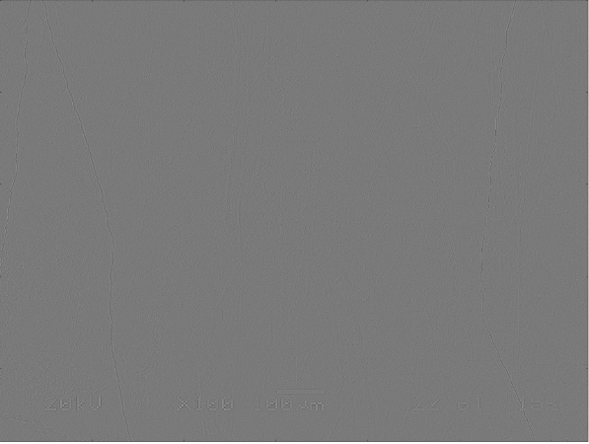
\includegraphics[width=.9\textwidth]{Laplace}
	\caption{Bordes usando Laplace}\label{fig:1.1.1}
	\end{subfigure}%
	\begin{subfigure}[c]{.33\linewidth}
	\centering\large 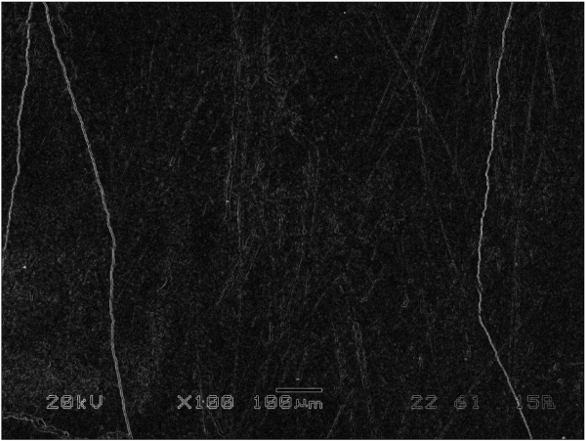
\includegraphics[width=.9\textwidth]{Prewitt}
	\caption{Bordes usando Prewitt}\label{fig:1.1.2}
	\end{subfigure}%
	\begin{subfigure}[c]{.33\linewidth}
	\centering\large 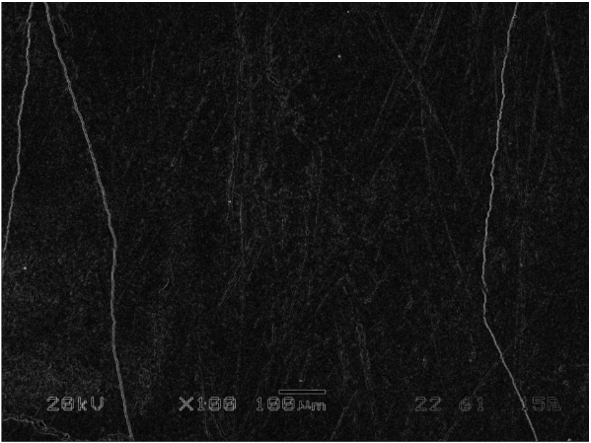
\includegraphics[width=.9\textwidth]{Scharr}
	\caption{Bordes usando Scharr}\label{fig:1.1.3}
	\end{subfigure}%
		
	\begin{subfigure}[c]{.33\linewidth}
	\centering\large 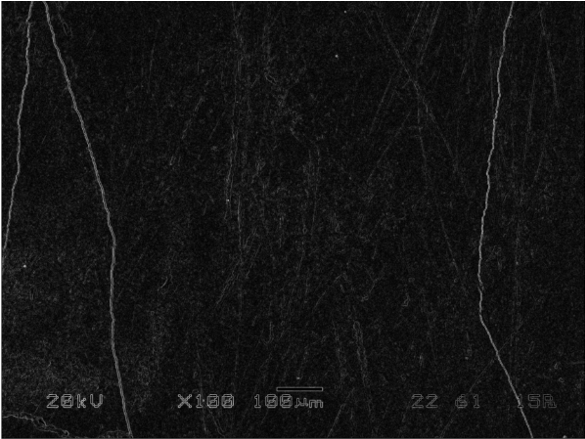
\includegraphics[width=.9\textwidth]{Sobel}
	\caption{Bordes usando Sobel}\label{fig:1.1.4}
	\end{subfigure}%
	\begin{subfigure}[c]{.33\linewidth}
	\centering\large 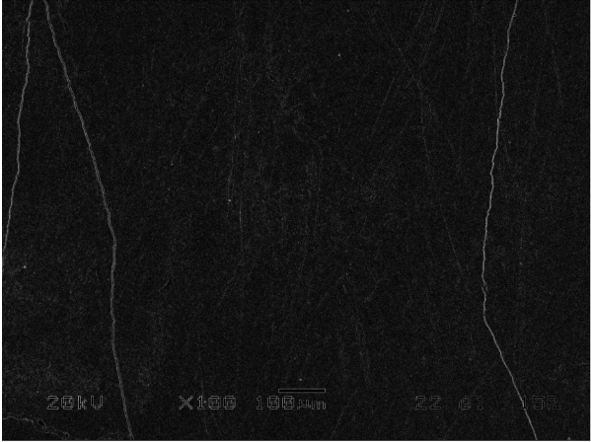
\includegraphics[width=.9\textwidth]{Roberts}
	\caption{Bordes usando Roberts}\label{fig:1.1.5}
	\end{subfigure}%	
	\begin{subfigure}[c]{.33\linewidth}
	\centering\large 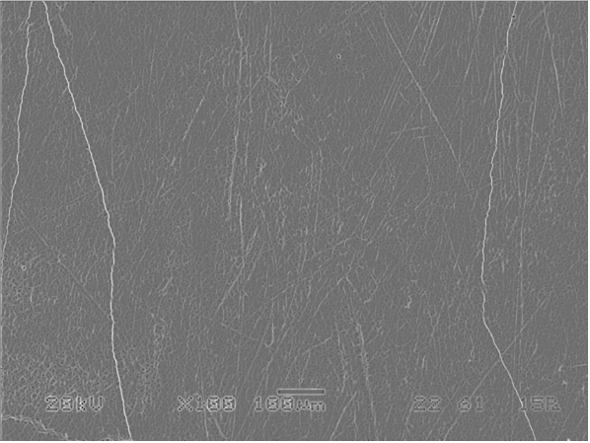
\includegraphics[width=.9\textwidth]{HessianaAutoLargos}
	\caption{Bordes usando HessianaAutoLargos}\label{fig:1.1.6}
	\end{subfigure}%
	
	\begin{subfigure}[c]{.33\linewidth}
	\centering\large 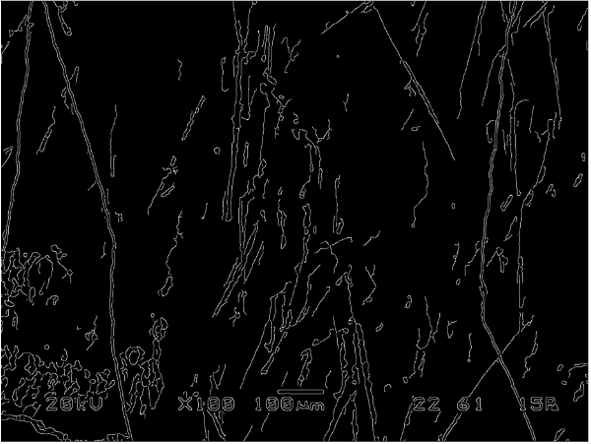
\includegraphics[width=.9\textwidth]{CannyP}
	\caption{Bordes usando CannyP}\label{fig:1.1.7}
	\end{subfigure}%
	\begin{subfigure}[c]{.33\linewidth}
	\centering\large 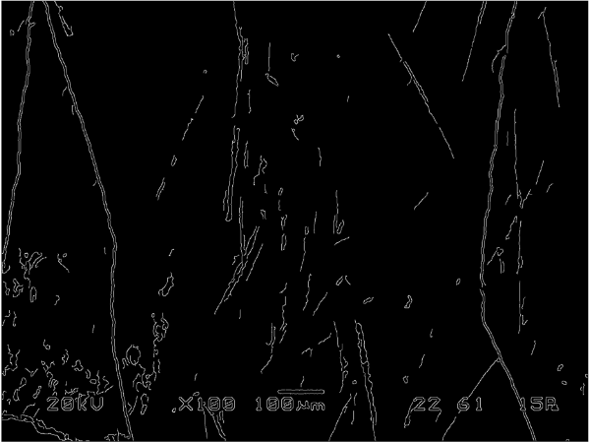
\includegraphics[width=.9\textwidth]{Canny}
	\caption{Bordes usando Canny}\label{fig:1.1.8}
	\end{subfigure}%	
	\begin{subfigure}[c]{.33\linewidth}
	\centering\large 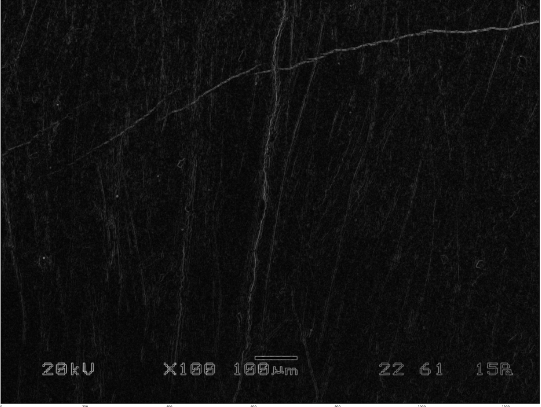
\includegraphics[width=.9\textwidth]{Kirsch}
	\caption{Bordes usando Kirsch}\label{fig:1.1.9}
	\end{subfigure}	
	
	\begin{subfigure}[c]{.33\linewidth}
	\centering\large 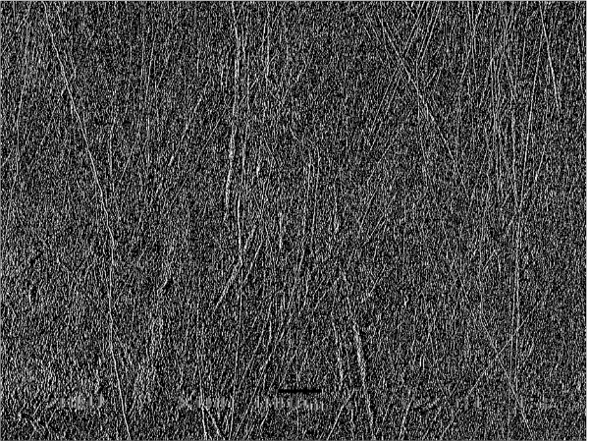
\includegraphics[width=.9\textwidth]{GaborI}
	\caption{Bordes usando Gabor filtro imaginario}\label{fig:1.1.10}
	\end{subfigure}%	
	\begin{subfigure}[c]{.33\linewidth}
	\centering\large 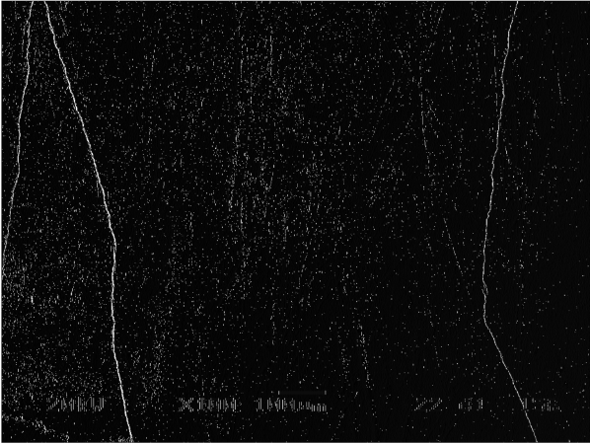
\includegraphics[width=.9\textwidth]{GaborR}
	\caption{Bordes usando Gabor filtro real}\label{fig:1.1.11}
	\end{subfigure}

\caption{Resumen visual filtros usados.}\label{fig:1.1}
\end{figure}






\begin{figure}

	\begin{subfigure}[c]{.55\linewidth}
	\centering\large 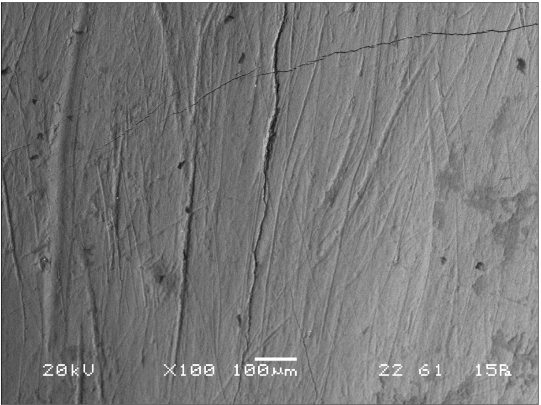
\includegraphics[width=.9\textwidth]{Imagen}
	\caption{Imagen original}\label{fig:2.1.1}
	\end{subfigure}%
	\begin{subfigure}[c]{.55\linewidth}
	\centering\large 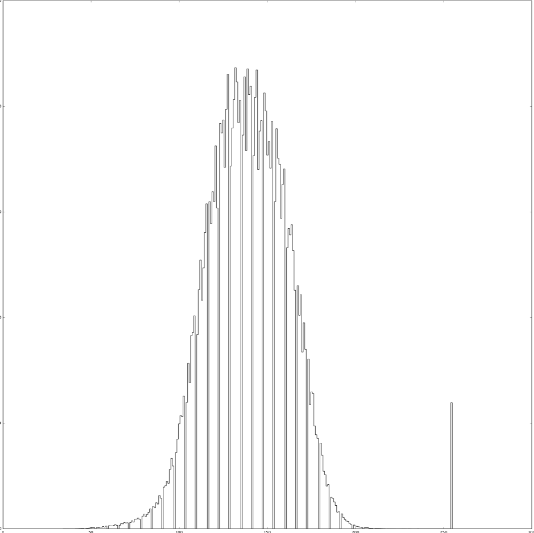
\includegraphics[width=.9\textwidth]{ImagenHist}
	\caption{Histograma imagen original}\label{fig:2.1.2}
	\end{subfigure}%
	
	\begin{subfigure}[c]{.55\linewidth}
	\centering\large 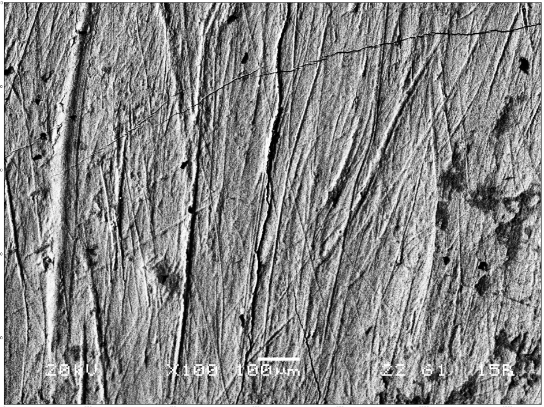
\includegraphics[width=.9\textwidth]{Equalized}
	\caption{Imagen ecualizada}\label{fig:2.1.3}
	\end{subfigure}%	
	\begin{subfigure}[c]{.55\linewidth}
	\centering\large 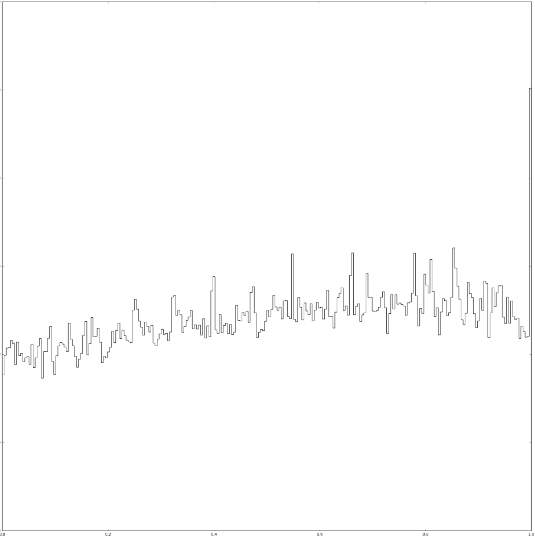
\includegraphics[width=.9\textwidth]{Histograma_Equali}
	\caption{Histograma imagen ecualizada}\label{fig:2.1.4}
	\end{subfigure}%
	\caption{Pasos del procesado parte uno.}\label{fig:2.1}

\end{figure}
 
	

\begin{figure}
	\begin{subfigure}[c]{.49\linewidth}
	\centering\large 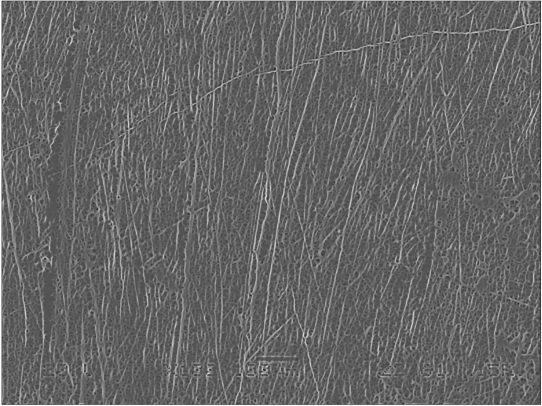
\includegraphics[width=.9\textwidth]{HessianaPaso2}
	\caption{Autovectores largos.}\label{fig:2.1.5}
	\end{subfigure}%
	\begin{subfigure}[c]{.49\linewidth}
	\centering\large 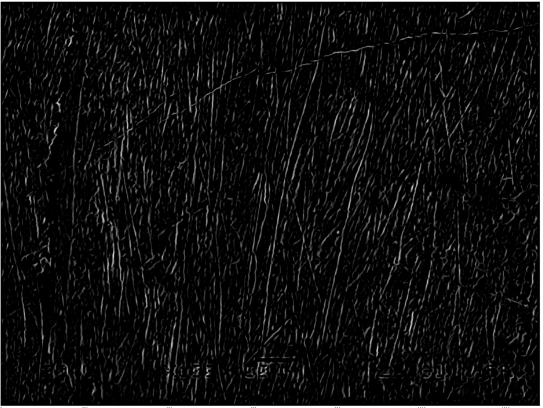
\includegraphics[width=.9\textwidth]{HessianaPaso2MenosFOndo}
	\caption{Hessiana menos fondo.}\label{fig:2.1.6}
	\end{subfigure}%
	
	\begin{subfigure}[c]{.49\linewidth}
	\centering\large 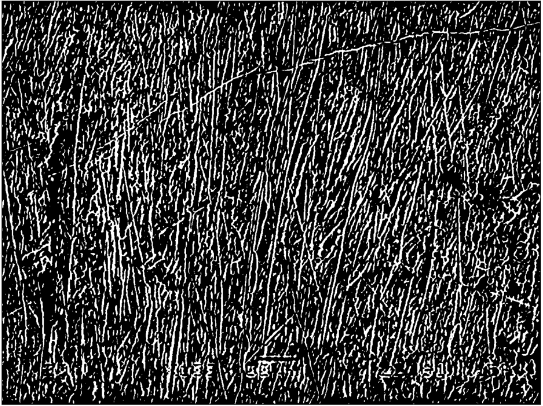
\includegraphics[width=.9\textwidth]{MenosFondoBinarizada}
	\caption{Binarizado.}\label{fig:2.1.7}
	\end{subfigure}%	
	\begin{subfigure}[c]{.49\linewidth}
	\centering\large 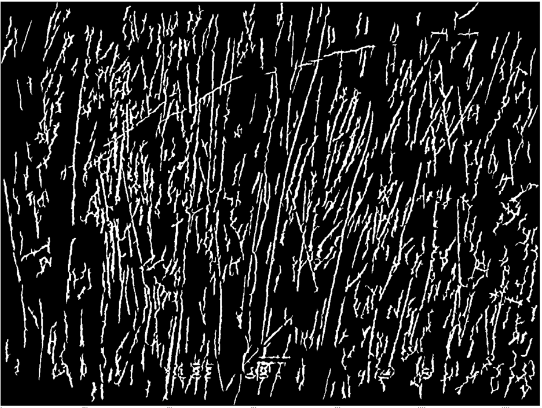
\includegraphics[width=.9\textwidth]{BinarizadaSinRuido}
	\caption{Binarizada sin ruido.}\label{fig:2.1.8}
	\end{subfigure}%	
	
	\begin{subfigure}[c]{.49\linewidth}
	\centering\large 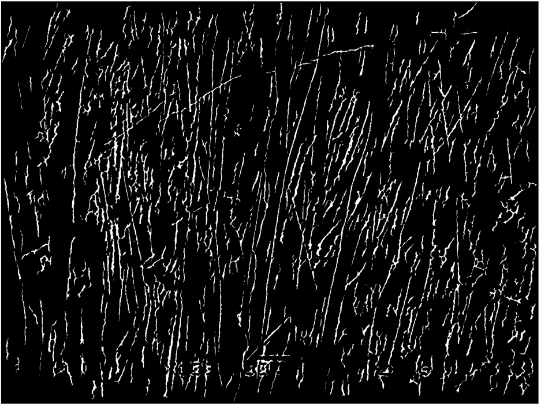
\includegraphics[width=.9\textwidth]{SinRuidoErosionada}
	\caption{Erosionado.}\label{fig:2.1.9}
	\end{subfigure}%	
	\begin{subfigure}[c]{.49\linewidth}
	\centering\large 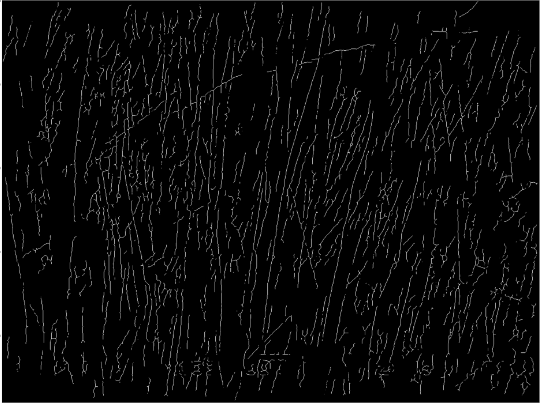
\includegraphics[width=.9\textwidth]{ErosionadaEsqueletonizada}
	\caption{Esqueletonizado de la erosión.}\label{fig:2.1.10}
	\end{subfigure}%	
		
	\begin{subfigure}{.49\linewidth}
	\centering\large 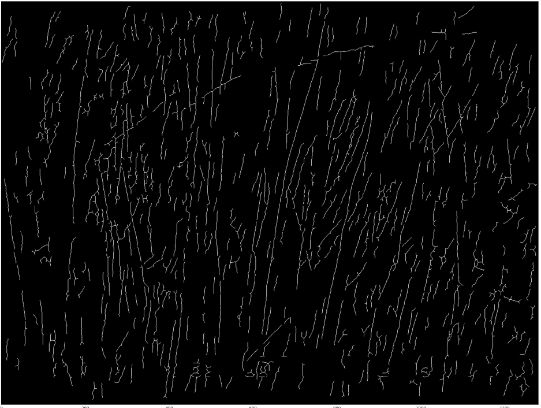
\includegraphics[width=.9\textwidth]{EsqueletonizadaSinRuido}
	\caption{Esqueletonizada sin ruido}\label{fig:2.1.11}
	\end{subfigure}%
	\caption{Pasos del procesado parte dos.}\label{fig:2.2}

\end{figure}

\begin{figure}

	\begin{subfigure}{.99\linewidth}
	\centering\large 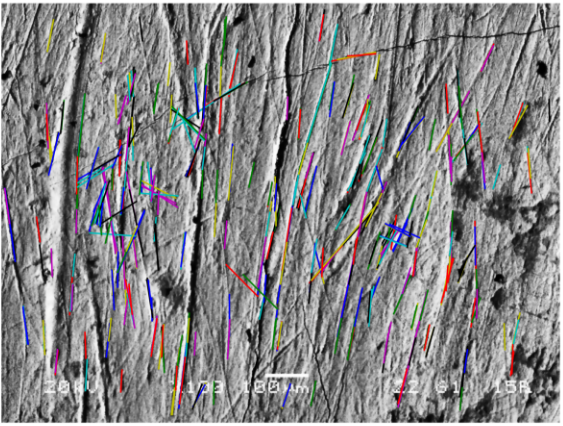
\includegraphics[width=.9\textwidth]{SegmentosSinUnir}
	\caption{Segmentos detectados}\label{fig:2.1.12}
	\end{subfigure}%
	
	\begin{subfigure}{.99\linewidth}
	\centering\large 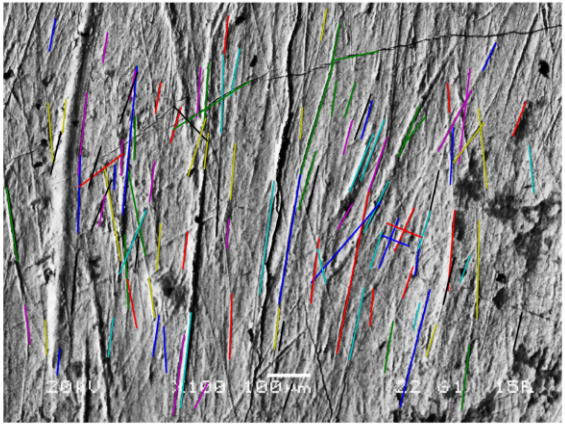
\includegraphics[width=.9\textwidth]{LineasReales}
	\caption{Segmentos reales}\label{fig:2.1.13}
	\end{subfigure}%
	
\caption{Pasos del procesado parte tres.}\label{fig:2.3}
\end{figure}
